\documentclass{article}

\usepackage[top=2.5cm,left=2.5cm,right=2.5cm,bottom=2.5cm]{geometry}
\usepackage[utf8]{inputenc}
\usepackage[T1]{fontenc}
\usepackage[francais]{babel}
\usepackage{graphicx}

\title{Stage chez Let There Be Light \\ \large Rapport d'étonnement}
\date{23 Janvier 2018}
\author{Baptiste \bsc{Saclier} \and Exia A3}

\begin{document}

\maketitle

\vspace{3cm}

\tableofcontents

\clearpage

\section{Let There Be Light}

La société Let There Be Light (ou LTBL) est un société qui réalise des dispositifs interactifs pour pour l'événementtiel, la communication et la culture.
Elle fut fondée en 2014 par Benjamin \bsc{Petit} et Antoine \bsc{Vanel} sous le nom de Beam'Art.
En 2016, elle change de nom et de status pour devenir l'entreprise que l'on connait actuellement.
Aujourd'hui Mr \bsc{Petit} en est le seul dirigeant.

%TODO Historique de l'entreprise

\subsection{Structure}

Let There Be Light est, sur la majorité des projets, un soustraitant de la société Vendredi 4.
Vendredi 4 est une société de communication spécialisée dans l'interaction.
Elle délegue le travail de développement à LTBL sur la majorité de ses projets.
Les contrats sont obtenus par Sylvie \bsc{Madamour}, la charte graphique du projet est alors composée par Vendredi 4.
LTBL intervient sur l'intégration de cette charte graphique dans des installations intéractives dans des salons au des showrooms.

Les équipes de Vendredi 4 et de LTBL sont assez réduite.
L'éfféctif de Vednredi 4 est donc de 3 employés quand LTBL compte un employé (Mr \bsc{Petit}) et un prestataire (Mr \bsc{Limoge})

\begin{figure}[h]
    \centering
    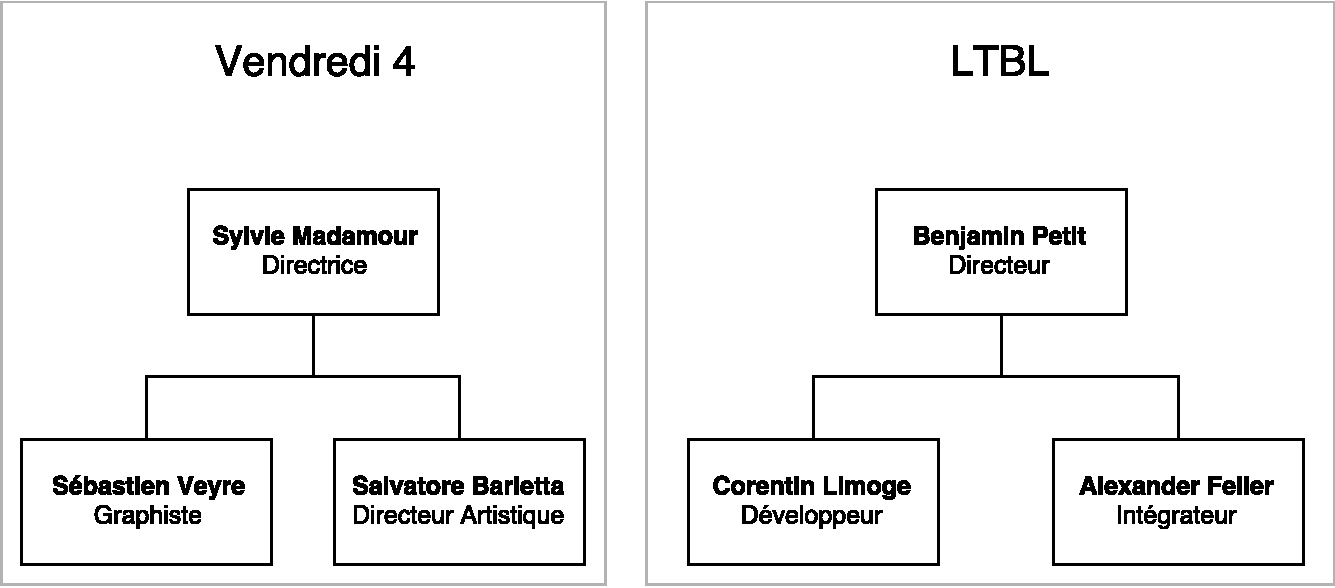
\includegraphics[scale=0.7]{Structure-LTBL.pdf}
    \caption{Structure de LTBL et Vendredi 4}
\end{figure}

Les deux entreprises sont trés liés, elles partagent les même locaux et communiqument beaucoup ensemble sur les projets en cours et à venir.

On retrouve alors Benjamin \bsc{Petit}, le gérant, et Corentin \bsc{Limoge} du coté LTBL.
Benjamin s'occupe des conseils et de la gestion de l'entreprise.
Il s'occupe aussi de l'aspect technique des installations par le choix des technologies de pointage et d'affichage.
Corentin est employé par LTBL mais dispose d'un status d'auto-entrepreuneur, on peut alors le considèrer comme un prestataire.
Corentin est en charge du développement des applications qui seront éxécutés sur les installations.

Du coté Vendredi 4 on retrouve Sylvie \bsc{Madamour}, la directrice, Salvatore \bsc{Barletta}, directeur artistique, et Sébastien \bsc{Veyre}, graphiste.
Sylvie est en charge des contrats, devis et de la communication avec les clients.
Salvatore est directeur artistique chez vendredi 4, il s'occupe de concevoir et présenter les design des installations aux clients.
Sébastien est graphiste et est en charge de représenter les futurs interfaces des installations mais aussi de travailler sur des rendus en Motion Design pour donner un premier aperçu de la futur application pour les clients et les intégrateurs.

\subsection{Projets}

Les deux entrprises travailleur ensemble pour proposer des services suivants :

\begin{itemize}
    \item Conseils téchniques
    \item Conseils en intéraction
    \item Design graphique
    \item Développement d'applications intéractives
    \item Installations
\end{itemize}

Ainsi, les deux entreprises peuvent suivre la production d'une application intractive de sa conception jusuqu'a son installation.

\medskip

Les projets suivi par LTBL sont les suivants :

\paragraph{Dispositifs de présentation intéractifs} Le plus souvent utilisés dans les salons et showrooms, les dispositifs intéractifs permettent une présentation des produits de manière ésthétique.
L'objectif de LTBL est donc de concevoir cette installation.
Cela passe par la conception du système phisique est des composants requis maus aussi par la conception et le développement de l'interface utilisateur qui doit être réactive et esthetique.
La majorité de ce type de projet est la présentation d'informations sur un produit sur un écran tactile sous forme de table tactile.

\paragraph{Vidéo Mapping} Le plus souvent présenté lors d'événements, le vidéo mapping consiste en la projection d'une image déformée sur une structure pouavnt être un batiment ou une installation spécifique.
Cette image utilise une représentation de la structure pour se déformer et épouser sa forme lors de la projection.
Ce type d'installation permet, au travers de jeux de lumière et d'illusions, de donner vie a la structure ou au batiment.
On retrouve ce type d'installation à la fête des lumières de Lyon par exemple.

\paragraph{Conseils technique ou en interaction} Fort de son experiance dans le domaine de l'intéractivité, LTBL peut aussi donner des conseils en interactivité dans le cadre de projets cités plus haut.

%TODO Fêtes des lumières

\subsubsection{Clients}

Les clients de LTBL et de Vendredi 4 sont, le plus souvent, de la région rhône alpes mais peuvent aussi être en région parisienne.
Ces clients sont des PME ou des grands groupes désirant de nouvelles installations intéractives pour leurs showrooms.
Au travers de ces installations, ils peuvent montrer leur produit de manière esthétiques a leurs clients.
Les showrooms ne sont pas les seuls installations organisés par LTBL, on retrouve aussi des présentation de produits pour les salons ou l'affichage de données pour la productivité dans les bureaux.

%TODO Liste des clients
%TODO proposition de projets a des événements

\section{Intégration}

Mon intégration dans l'entrprise c'est faite tres rapidement.

J'ai commencé par passer l'entretien le 27 Novembre qui c'est très bien passé.
J'ai découvert une équipe réstreinte de 2 personnes sympatiques et ayant des projets intéressants.
On m'a informé sur les objectifs de mon stage.

J'ai intégré l'entreprise le 9 Janvier.
J'ai alors découvert ma première mission, le développement d'une application Electron pour afficher les produits de l'entreprise Biomérieux.

La première journée fut une journée de mise en place ou j'ai pu acceder aux infrastructure de LTBL.
J'ai eu acces à leur dépot de code sur BitBucket et les conversations de groupe de LTBL et Vendredi 4 sur Slack.
Enfin, j'ai pu me joindre au Trello mis en place pour le projet que j'ai à faire.

Durant ma première semaine, je me suis familiarisé avec ma première mission et les technologies qui l'entourent comme Electron et les WebComponents.
Je conaissait déjà Electron, une solution de développement d'application natives avec des outils Web.
En revanche je ne connaissait pas les Webcomponents, un nouveau standard web permettant de concevoir des tags HTML personnalisés.
Par contre, j'avais déjà utilisé des framework Javascript avec la même philosophie comme VueJS et Angular;
Avec ces compétences que je possèdait déjà et l'expériance de Corentin, j'ai pu apprendre ce nouveau système en une journée.

Le début de ma mission fut assez difficile car, même si je comprenait les bjectifs, aucun cahier des charges n'a formellement été rédigé.
Je me suis donc appuyé sur la vidéo en Motion Design de Sébastien pour en déduir les fonctionnalités à implémenter.
De plus, mon maitre de stage étant aux Etats unis pour le CES de Las Vegas, je ne pouvait pas lui parler sur mes horaires de travail ce qui rend la conception de la solution difficile.

En conclusion, les premières semaines de mon stage se sont très bien passé et je me suis intégré dans cette entreprise plus rapidement que dans les autres stages que j'ai éfféctué.
Cela est surement due à l'ambiance bonne enfant et sympatique des équipes et aussi de l'éfféctif réduit.

\section{Etonnement}

Durant les premières semaines de mon stage j'ai eu l'occasion de découvrir cette entreprise et ses particularités par rapport aux autres entreprises que j'ai intégré.

\paragraph{Ambiance} L'éfféctif réduit de l'etreprise (2 chez LTBL et 3 chez Vendredi 4) permettent de s'intègrer très facilement a l'équipe et de communiquer plus aisément.
Il n'est même plus nécéssaire d'utiliser le Slack mis en place pour communiquer sur les projets sur les heures de travail.
De plus, les employés de l'entreprises sont passionnés par leur domaine et cela se sent.
Ils sont très qualifiés et curieux dans la technologie et m'on déjà fait découvrir de nombreuses choses.
Enfin, la curiosité de l'équipe les amènent a découvrir de nouvelles technologies même si cela n'est pas l'objectif premier du projet.
Par exemple, l'entreprise à investi dans une imprimante 3D pour éxpérimenter cette technologie pouvant être utilise pour la fabrication de structure ou de boitier.

\paragraph{Deadlines} J'ai remarqué que LTBL est en charge de courts voir tres courts projets qui ne sont pas maintenus sur le long terme.
Ma première mission est un projet de développement d'application sunr un seul mois.
En effet, la première présentation du produit s'éfféctuera le 7 février.
La faible maintenance des projets de LTBL est justifiée par le fait qu'ils contrôlent leurs installations du hardware jusqu'au software par le choix des technologies a utiliser et l'installation chez le client.
Ainsi, une fois que l'installation fonctionne, il n'est plus nécéssaire de s'en occuper pour qu'elle fonctionne pendant plusieurs mois voir années.

\paragraph{Locaux \& matériel} Les locaux de LTBL sont assez petit et sont partagés par les deux entreprises.
Ces locaux sont composés de 2 bureaux, une salle principale avec mezzanine et une salle de pause.
Cela suffit pour les équipes mais la periode à laquelle je suis arrivée est un periode de livraison pour des projets de tables tactiles.
Ainsi, des écrans tactile de grande taille on été livrés pour pouvoir tester en conditions réel les applications.
De plus, au retour de la fète des lumières de Hong Kong, beaucoup de materiel comme des barres de LED et des vidéosprojecteurs ont été stockés dans les locaux.

\section{Missions}

\subsection{Biomérieux}

\subsection{Installation au salon de l'entreprise du futur}

\subsection{Blind Test}

\section{Missions à venir}

\section{Conclusion}

\section{Bilan}

\end{document}